% generated by tools/report/gen_grass.py: do not edit
\newcommand{\grasscard}{%
\needspace{12cm}
\begin{center}
\fcolorbox{black!30}{white}{\begin{minipage}{0.975\linewidth}\centering\vspace{0.6mm}
\begin{minipage}[b]{0.37\linewidth}\centering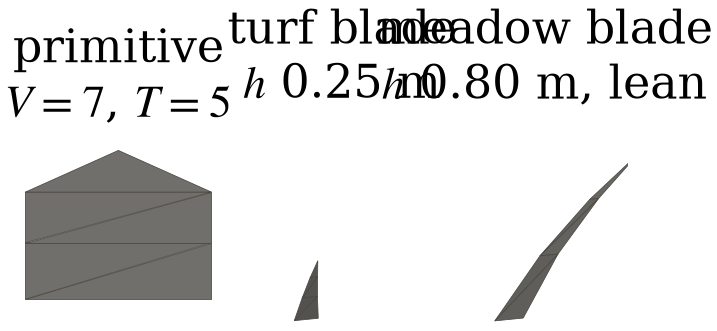
\includegraphics[width=\linewidth]{figures/img/shapes/grass_blade.png}\\{\footnotesize (a) primitive and two instances}\end{minipage}\hfill
\begin{minipage}[b]{0.17\linewidth}\centering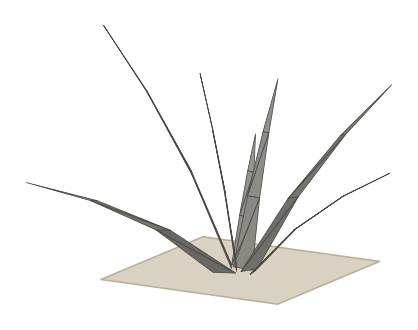
\includegraphics[width=\linewidth]{figures/img/shapes/grass_tuft.png}\\{\footnotesize (b) one tuft}\end{minipage}\hfill
\begin{minipage}[b]{0.42\linewidth}\centering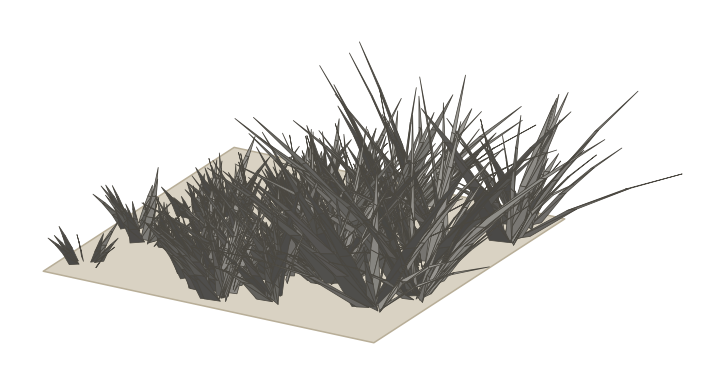
\includegraphics[width=\linewidth]{figures/img/shapes/grass_patch.png}\\{\footnotesize (c) a 1.6\,m patch: turf (left), meadow (right)}\end{minipage}\\[1.5mm]
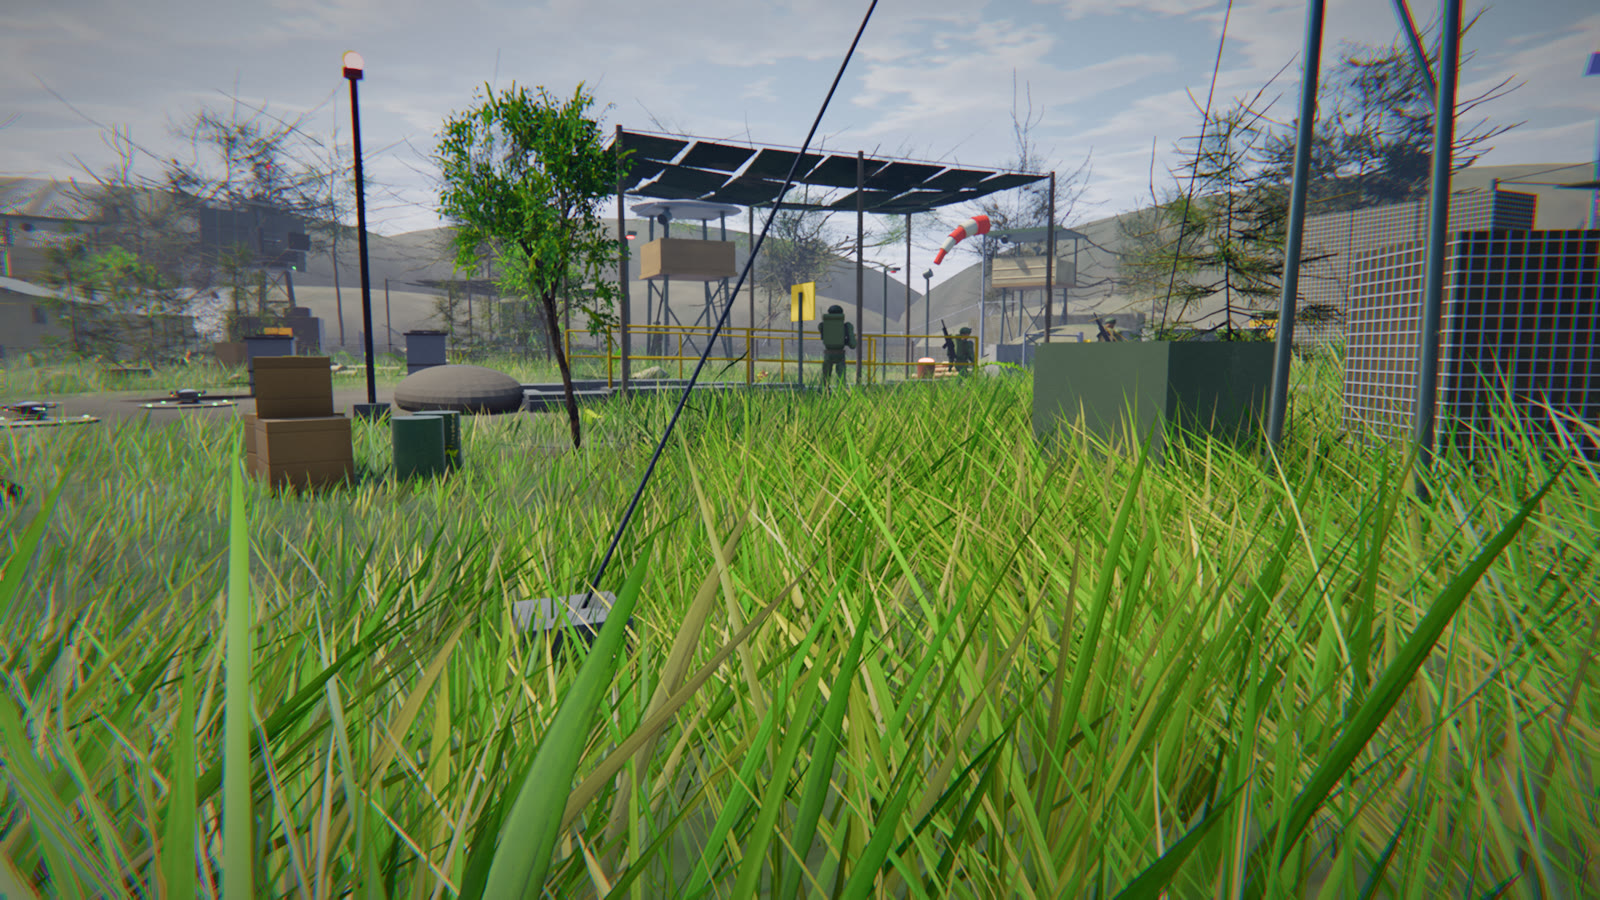
\includegraphics[width=\linewidth,height=4.2cm,keepaspectratio]{figures/img/scene/m6_grass_close.jpg}\\{\footnotesize (d) the same blades rendered in the scene (EPIC, textured, alpha-to-coverage)}
\\[0.8mm]{\fontsize{7}{8.5}\selectfont \primchipn{grassblade}{450\,000} \quad blades over the whole base, one instanced draw call per visible cell}\vspace{0.6mm}\end{minipage}}
\captionof{figure}{Grass field. (a--c) are drawn in the key colour from the primitive and the rules of \code{rendering/Grass.cpp} (widths drawn $\times4$, single blades $\times9$, wind left out).}\label{fig:d-grass}
\end{center}\vspace{-3mm}
\noindent\textbf{Grass field.}\label{des:grass} One primitive, instanced on the \ab{469}{GPU}: the grass is not a scene-graph part and is not counted in the \sceneParts{} parts. Its rules:
\begin{center}\fontsize{7.5}{9}\selectfont\begin{tabularx}{\linewidth}{@{}>{\bfseries}lX@{}}\toprule
Primitive & grass blade (Section~\ref{sec:prims}): $V=7$, $T=5$, a folded strip of three rows and a tip\\
Blades & budget per preset: LOW 14\,000, HIGH 35\,000, ULTRA 140\,000, EPIC 450\,000\\
Tuft & 7--12 blades within 7\,cm of a centre; yaw $=$ the direction out from the centre; lean grows to the rim\\
Height & short turf 0.12--0.32\,m; tall meadow 0.50--0.90\,m where a large-scale noise says ``uncut''\\
Instance & per blade: root $(x,y,z)$, yaw, height, width, lean, seed (two \code{vec4} attributes)\\
Shape & width $\times(1-0.96t)$, bend $\propto\operatorname{mix}(t,t^2,0.3)$ along the lean plus wind gusts\\
Culling, \ab{470}{LOD} & 10$\times$10 cells; every blade within 26\,m, 40\,\% at 75\,m, 24\,\% past 120\,m (the kept blades widen)\\
Area & full density inside the 20\,m compound, 45\,\% on the apron to the base edge\\
\bottomrule\end{tabularx}\end{center}}
